\subsection{Sensoren}
\label{subsec:Sensoren}
Der grossteil der Sensorik wurde bereits während des Projekt 5 implementiert und in dessen Fachbericht dokumentiert. Die Dokumentation der bereits implementierten Sensoren wird in nachfolgendem Abschnitt inkludiert und darauf folgend die während der Bachelor-Thesis hinzugekommene Sensorik bzw. Ergänzungen in einem separaten Abschnitt erläutert.

\subsubsection{Ombrometer - Projekt 5}

\subsubsection*{\textbf{Ermittlung der Niederschlagsmenge}}
Dieses Unterkapitel befasst sich mit der Realisierung der Niederschlagsmessung. Diese soll nach einem Kipplöffelprinzip funktionieren und gemäss definierten Zielen eine Genauigkeit von $\pm$100 ml/$m^2$ aufweisen. Ausserdem soll als alternative zusätzlich ein Messbecher an der Wetterstation installiert werden, damit der Bauer die Niederschlagsmenge anhand einer Skala ablesen kann. In einem ersten Schritt soll das Kipplöffelprinzip näher erläutert und mit einem Selbstbau die Funktionsweise getestet werden. Anschliessend soll ein gekaufter Sensor die Wetterstation erweitern und die Implementation in der Firmware thematisiert werden. Zu guter Letzt soll die Validierung des Teilsystems folgen.
\subsubsection*{\textbf{Das Kipplöffelprinzip}}
Das Prinzip des Kipplöffels wird in Abbildung \ref{fig:Kipp} graphisch dargestellt.

\begin{figure}[h]
\centering
\includegraphics[width=0.8\linewidth]{graphics/Kipploeffel.png}
\caption{Darstellung des Kipplöffelprinzips}
\label{fig:Kipp}
\end{figure}

Abbildung \ref{fig:Kipp} zeigt das Kipplöffelprinzip. Der Kipplöffel (\glqq 3)\grqq) besteht im Grunde aus zwei Löffeln und ist in der Mitte drehbar mit dem Gehäuse befestigt (\glqq 4)\grqq). Regenwasser wird über eine Öffnung im Gehäusedeckel (Trichter, \glqq 1)\grqq) zum Kipplöffel befördert (\glqq 2)\grqq). Ist der Löffel mit Regenwasser gefüllt, so kippt dieser aufgrund des Gewichts und leert das Wasser über eine Öffnung im Gehäuseboden (\glqq 5)\grqq) aus. Durch die Kippung wird der andere Löffel in die Ausgangsposition bewegt und kann sich nun mit Wasser füllen. Mit der Hilfe von Reedkontakten und Magneten wird die Anzahl der Kippbewegungen gezählt. Die Niederschlagsmenge ergibt sich aus der Anzahl Kippbewegungen, multipliziert mit dem Volumen des Kipplöffels.
\newpage

\subsubsection*{\textbf{Die Realisierung des Niederschlagsmengensensors}}
Um die Funktionsweise des Niederschlagsmengensensors  zu testen, wird, wie im Pflichtenheft festgehalten, dieser in einem ersten Schritt selbst erstellt. Die Erstellung kann in vier Etappen unterteilt werden. Die erste Etappe ist die Erstellung des Kipplöffels. Die zweite Etappe folgt mit der Erstellung der Drehbaren Lagerung. Als dritte Etappe folgt der Trichter und die vierte und letzte Etappe widmet sich dem Gehäuse, wobei der Trichter ein Teil des Gehäuses darstellt. Das Gehäuse wird, bei verwendung der Eigenproduktion, erst im Projekt 6 mit dem Gehäuse der gesamten Wetterstation erstellt.
\paragraph{\textbf{Etappe 1: Realisierung des Kipplöffels}}
Wichtig für die Erstellung des Kipplöffels sind die Dimensionierung und die Materialwahl.
 
Das Material soll wetterbeständig, einfach bearbeitbar und günstig sein und eine möglichst glatte Oberfläche haben. Die möglichst glatte Oberfläche ist notwendig, damit das Wasser im Kipplöffel sich nicht an der Oberfläche festhält und somit gut abfliesst. Acrylglas erfüllt diese Bedingungen und ist in jedem Baumarkt erhältlich, weshalb es als Material gewählt wird.

Die Dimensionierung ist Abhängig von der gewählten Genauigkeit im Pflichtenheft. Damit eine Genauigkeit von $\pm$100 ml/$m^2$ erreicht werden kann, müssen beide Löffel des Kipplöffels bei genau 100 ml Fassungsvermögen kippen. Damit dies erreicht wird, kann man physikalisch die statische Gleichgewichtsbedingung aufstellen und daraus die Dimensionierung folgern. Dies ist jedoch ein sehr aufwändiger, komplizierter und zeitintensiver weg. Einfacher ist es, wenn der Kipplöffel extra zu gross dimensioniert und die Füllmenge im nachhinein justiert wird. Die Justierung erfolgt mittels einer in der Höhe verstellbaren Lagerung, sowie mit in der Höhe verstellbaren Schrauben im Gehäuseboden, welche die Neigung der Endposition des Kipplöffels beeinflusst. Ein weiterer Vorteil dieser Nachjustierung ist, dass auch eine andere Füllmenge einstellbar wäre.

\begin{figure}[h]
\centering
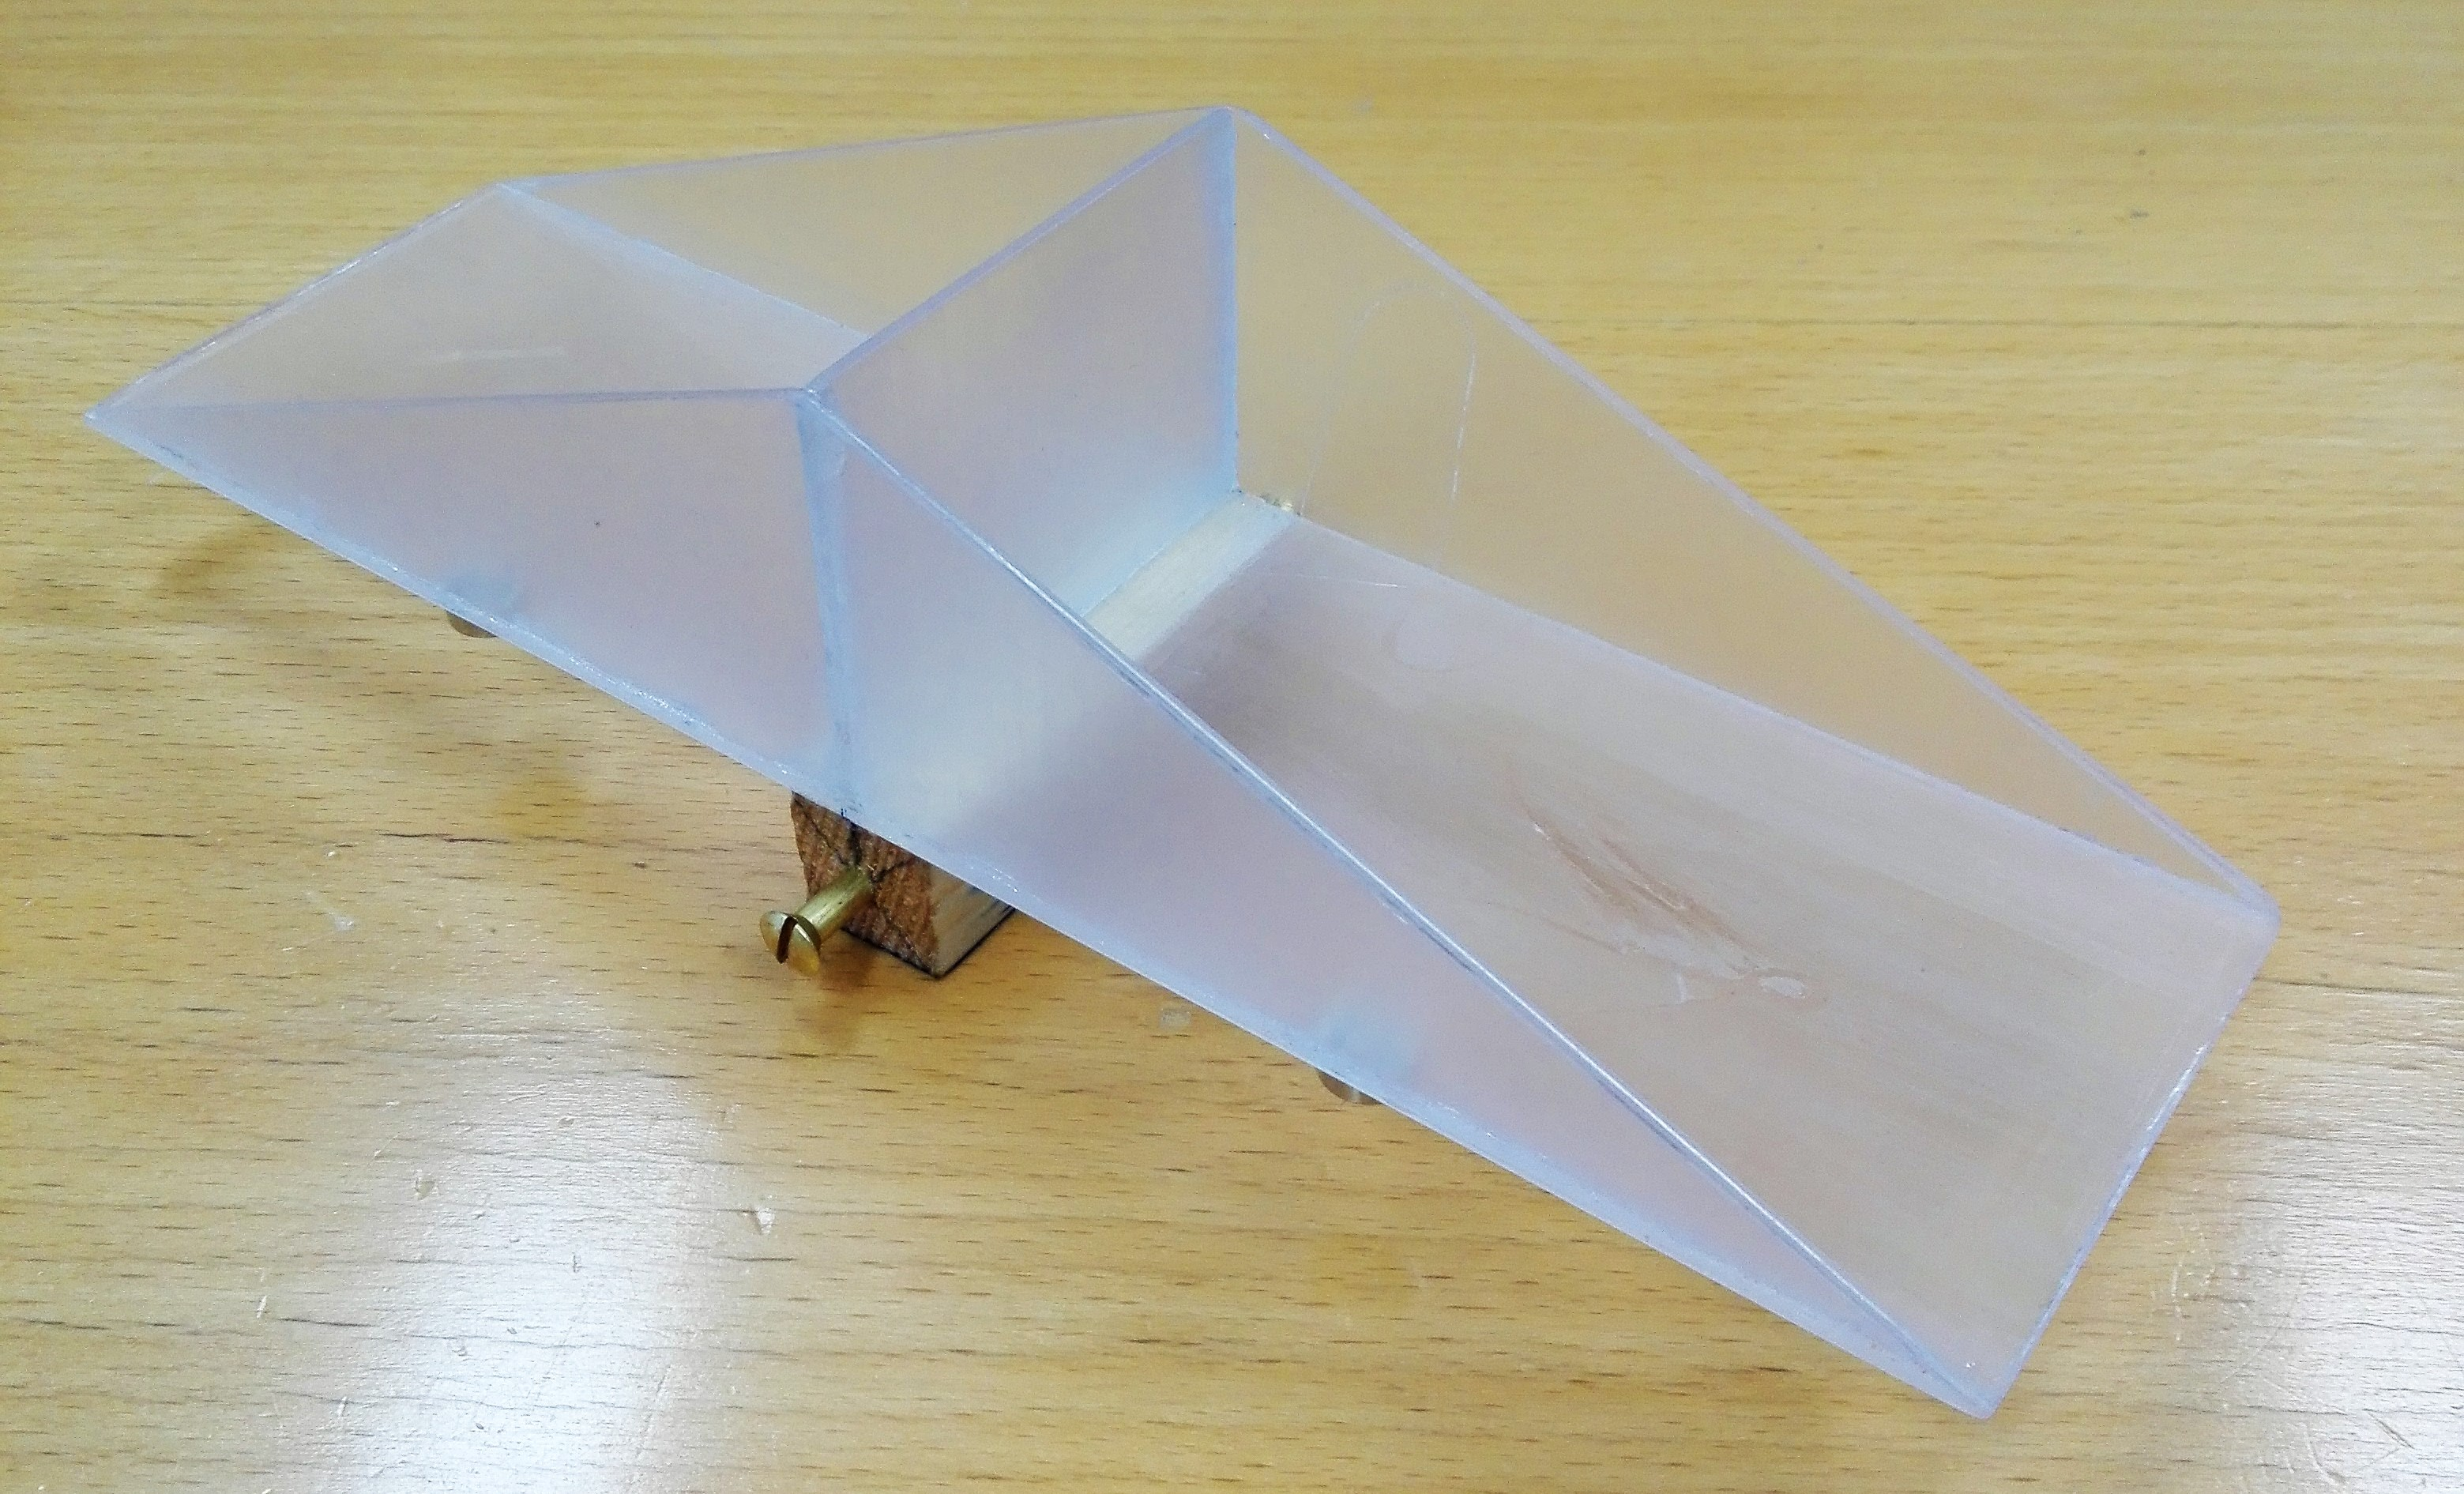
\includegraphics[width=0.8\linewidth]{graphics/Etappe1.jpg}
\caption{Selbsterstellter Kipplöffel.}
\label{fig:Etappe1}
\end{figure}

Abbildung \ref{fig:Etappe1} zeigt den selbsterstellten Kipplöffel aus Acrylglas. Die Drehachse ist mittig unter dem Kipplöffel befestigt und besteht aus einem Holzklotz mit je einer Schraube pro Seite.

\paragraph{\textbf{Etappe 2: Realisierung der drehbaren Lagerung}}
Die Drehbare Lagerung des Kipplöffels ist wichtig, damit der Kipplöffel auf beide Seiten kippen kann. Die Drehachse soll direkt unterhalb der Mitte des Kipplöffels befestigt sein um ein gleichmässiges Kippen zu ermöglichen. Die Höhe des Kipplöffels wird definiert durch die einstellbare Höhe der Drehachsenlagerung. 

Die Drehachse wird aus einem Stück Holz und zwei Schrauben gefertigt, wobei das Holz direkt am Kipplöffel befestigt wird. Die zwei Schrauben werden auf einem höhenverstellbarem Gerüst gelagert, so dass ein drehen möglich ist. Dieses Gerüst wird auch aus Holz gefertigt und enthält eine Metallische Fläche an der Kontaktstelle der zuvor erwähnten Schrauben, um aufkommende Reibkräfte zu verringern. Ausserdem ist dieses Gerüst höhenverstellbar über zwei mit Muttern feststellbaren Gewinden (für jede Seite eine). 

\begin{figure}[h]
\centering
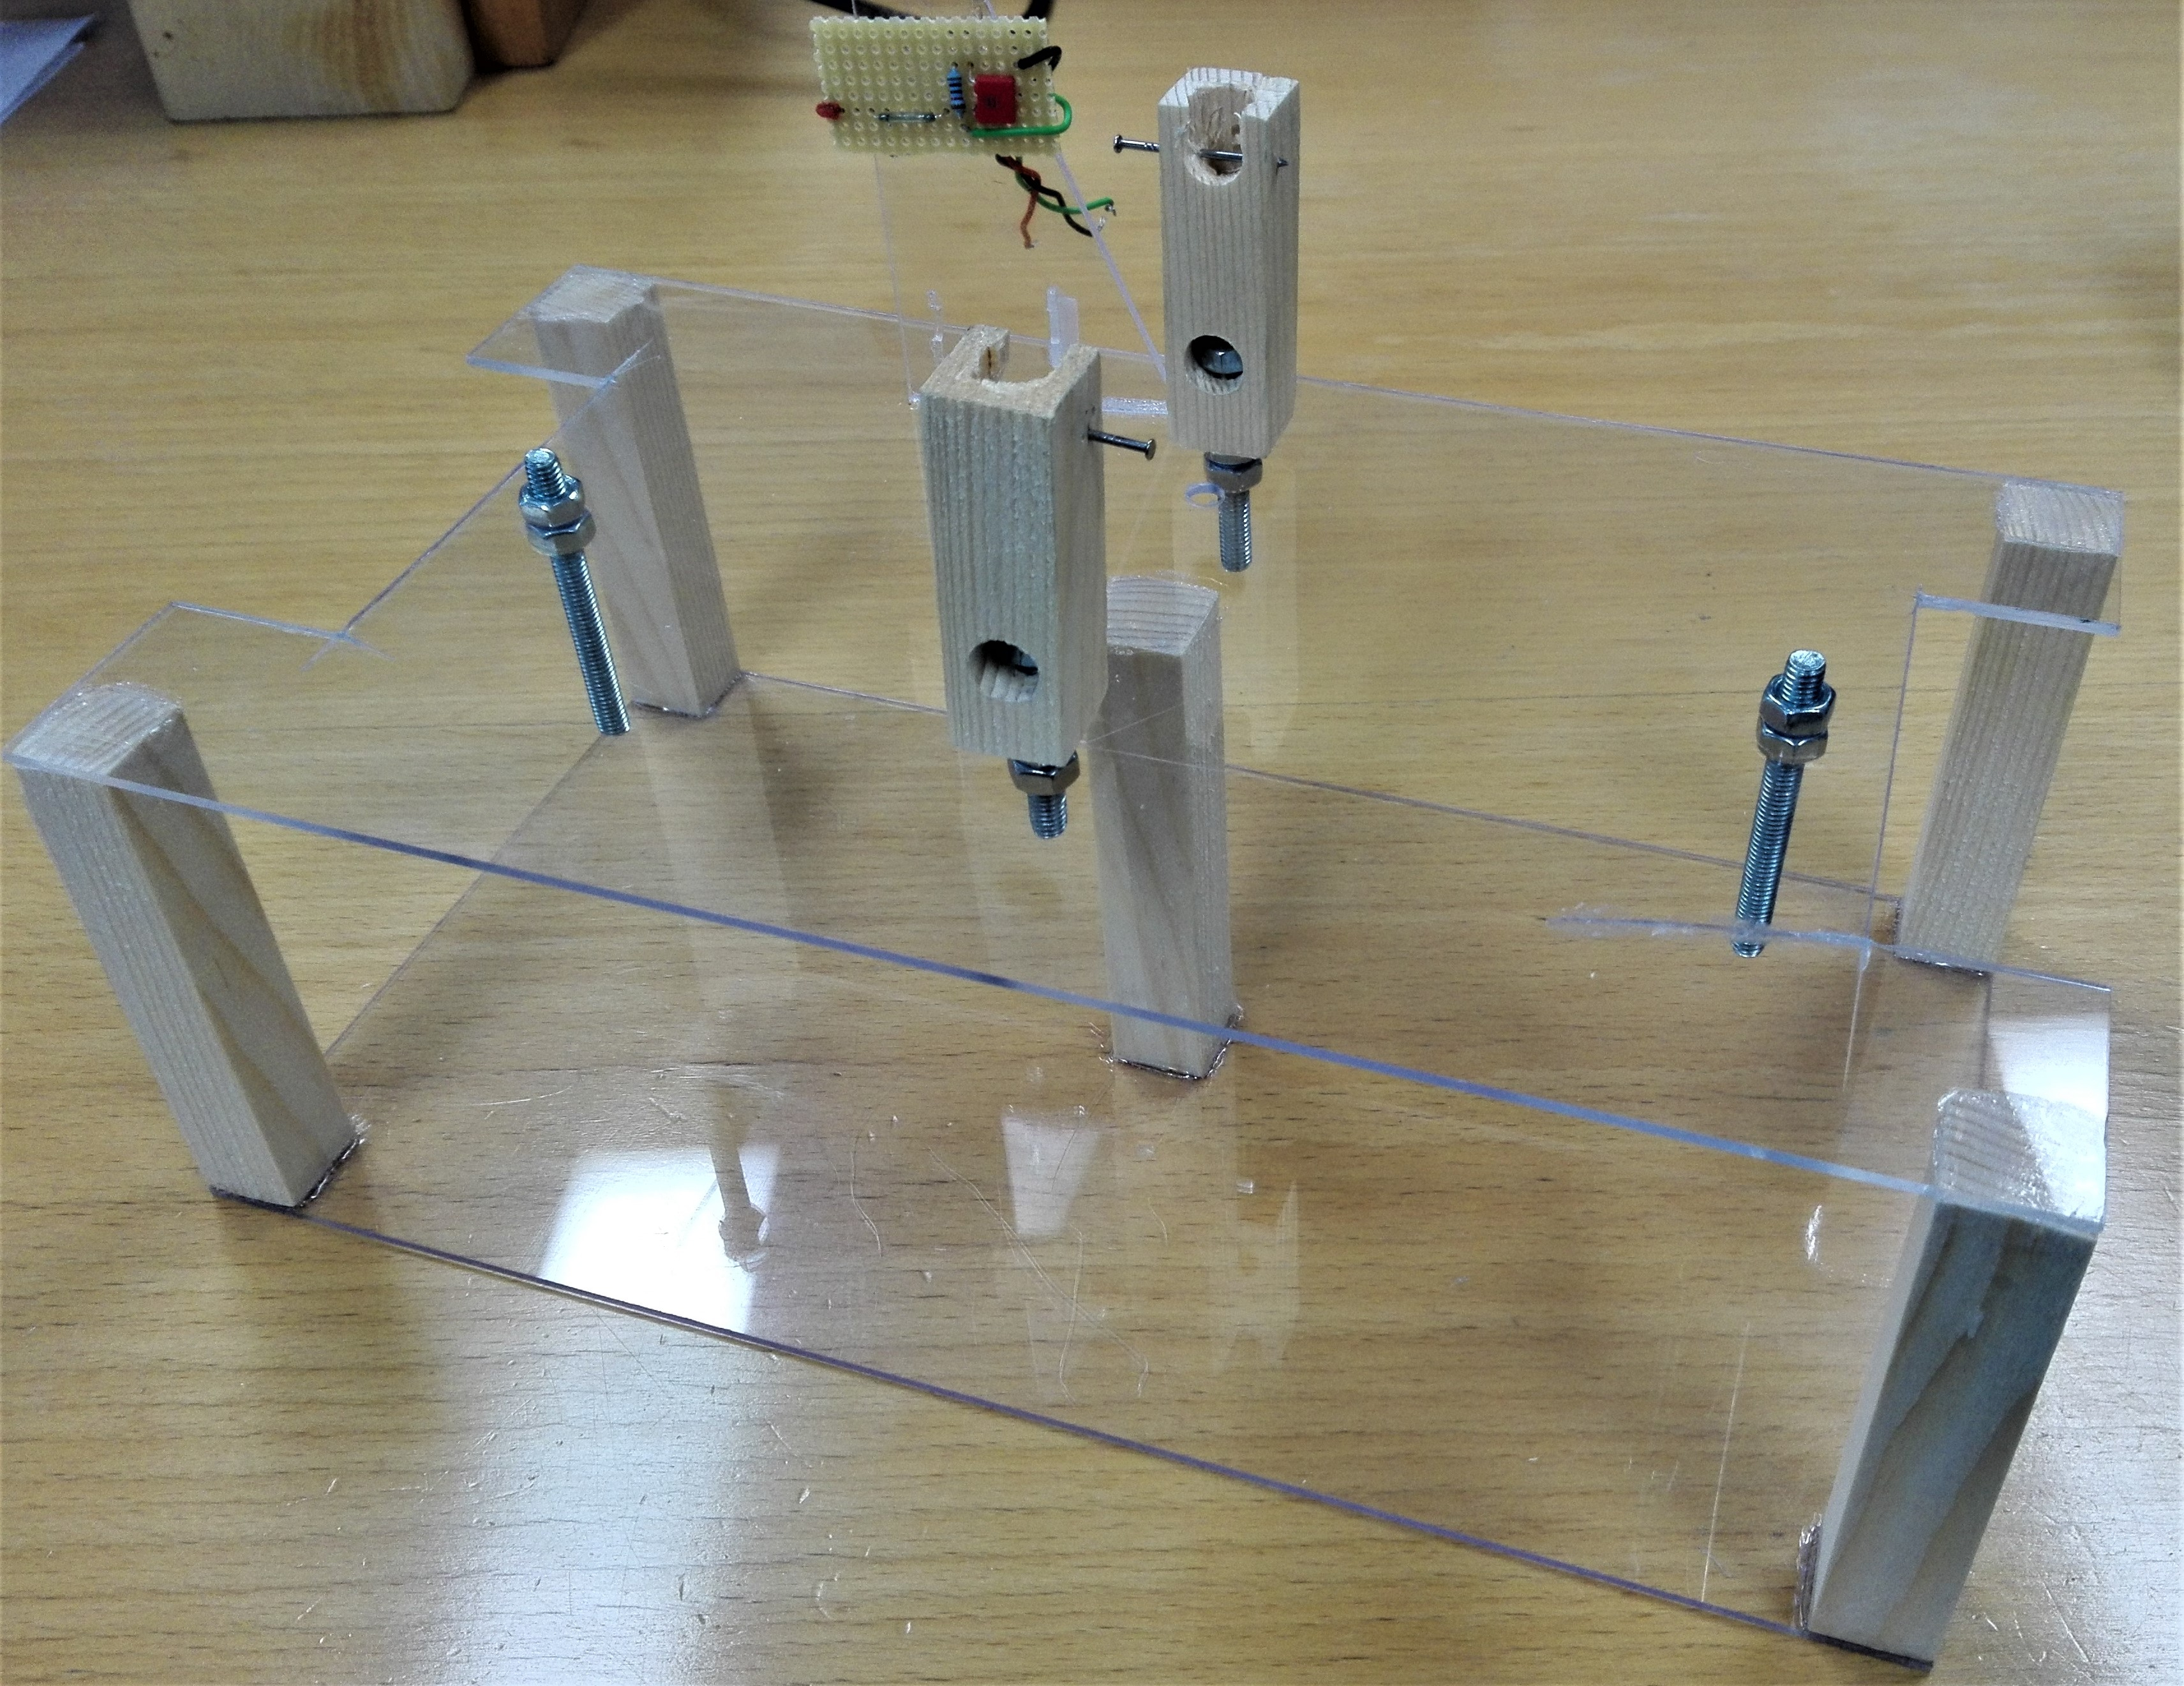
\includegraphics[width=0.8\linewidth]{graphics/Etappe2.jpg}
\caption{Selbsterstelltes Gerüst.}
\label{fig:Etappe2}
\end{figure}

Abbildung \ref{fig:Etappe2} zeigt das selbsterstellte Gerüst für die Höhenverstellbare, drehbare Lagerung des Kipplöffels. Es kann sowohl die Höhe des Kipplöffels, sowie dessen Neigung in den Endpositionen über Gewinden mit Muttern eingestellt werden. Die Schrauben des Kipplöffels kommen auf einen Stahlnagel zu liegen, womit Reibungsverluste gering gehalten werden.

\paragraph{\textbf{Etappe 3: Realisierung des Trichters}}
Der Trichter sorgt dafür, dass der Regen, welcher auf die Trichterfläche fällt, über der Mitte des Kipplöffels in den Löffel fliesst. Die Trichterfläche stellt gleichzeitig die Referenzfläche dar, da die gesamte Regenmenge dieser Fläche über den Kipplöffel erfasst wird. Ist diese Fläche von 1 $m^2$ abweichend, so muss in der Firmware ein Skalierungsfaktor implementiert werden, damit die Regenmenge wie gewünscht gemäss Pflichtenheft ermittelt werden kann. Der Trichter wird aus demselben Material gefertigt wie der Kipplöffel, da hier die gleichen Anforderungen gelten. Es sei angemerkt, dass der Trichter nur bei weiteren Verwendung des selbst erstellten Kipplöffels, zusammen mit dem Gehäuse der gesamten Wetterstation, erstellt wird.

\paragraph{\textbf{Etappe 4: Realisierung des Gehäuses}}
Das Gehäuse soll den Sensor vor ungewollten äusseren Einflüssen schützen, sowie umgebende Elektronik vor eventuellen Regenwasserspritzer. Ausserdem soll ein Schaltkreis mit Reedrelais implementiert werden, damit die Kippbewegungen von der Elektronik erfasst werden können. Es sei erwähnt, dass das Gehäuse nur bei weiteren Verwendung des selbst erstellten Sensors, zusammen mit dem Gehäuse der Wetterstation, konstruiert wird.

\paragraph{\textbf{Implementierung des Schaltkreises}}
Der Schaltkreis, welcher die Kippbewegungen feststellen soll, besteht im wesentlichen aus einem Reedrelais und einem Permanentmagneten. Das Reedrelais ist NO (Normally Open) und wirkt als stromkreisschliessender Schalter, sobald ein magnetisches Feld (z.B. das eines Permanentmagneten) sich in unmittelbarer Nähe befindet. Der Permanentmagnet wird auf dem Kipplöffel befestigt und das Reedrelais als Gegenstück an einem Fixpunkt in der Nähe. Wichtig dabei ist, dass das Reedrelais bei den Endpositionen des Kipplöffels nicht geschlossen ist, damit der Stromkreis geöffnet ist und Strom gespart werden kann. Das Reedrelais benötigt einen seriellen Widerstand, damit bei einem schliessen des Stromkreises kein Kurzschluss auftritt. Ausserdem soll ein Kondensator parallel zum Widerstand sein, um die Speisespannung zu glätten und so ein nutzbares Signal zu erhalten. Die Speisespannung stellt den Pegel für ein schliessen des Reedrelais, und somit auch für eine Kippbewegung dar. Um die Kippbewegungen zu zählen, kann somit entweder jede steigende oder jede fallende Flanke des Signals gezählt werden.  

\begin{figure}[h]
\centering
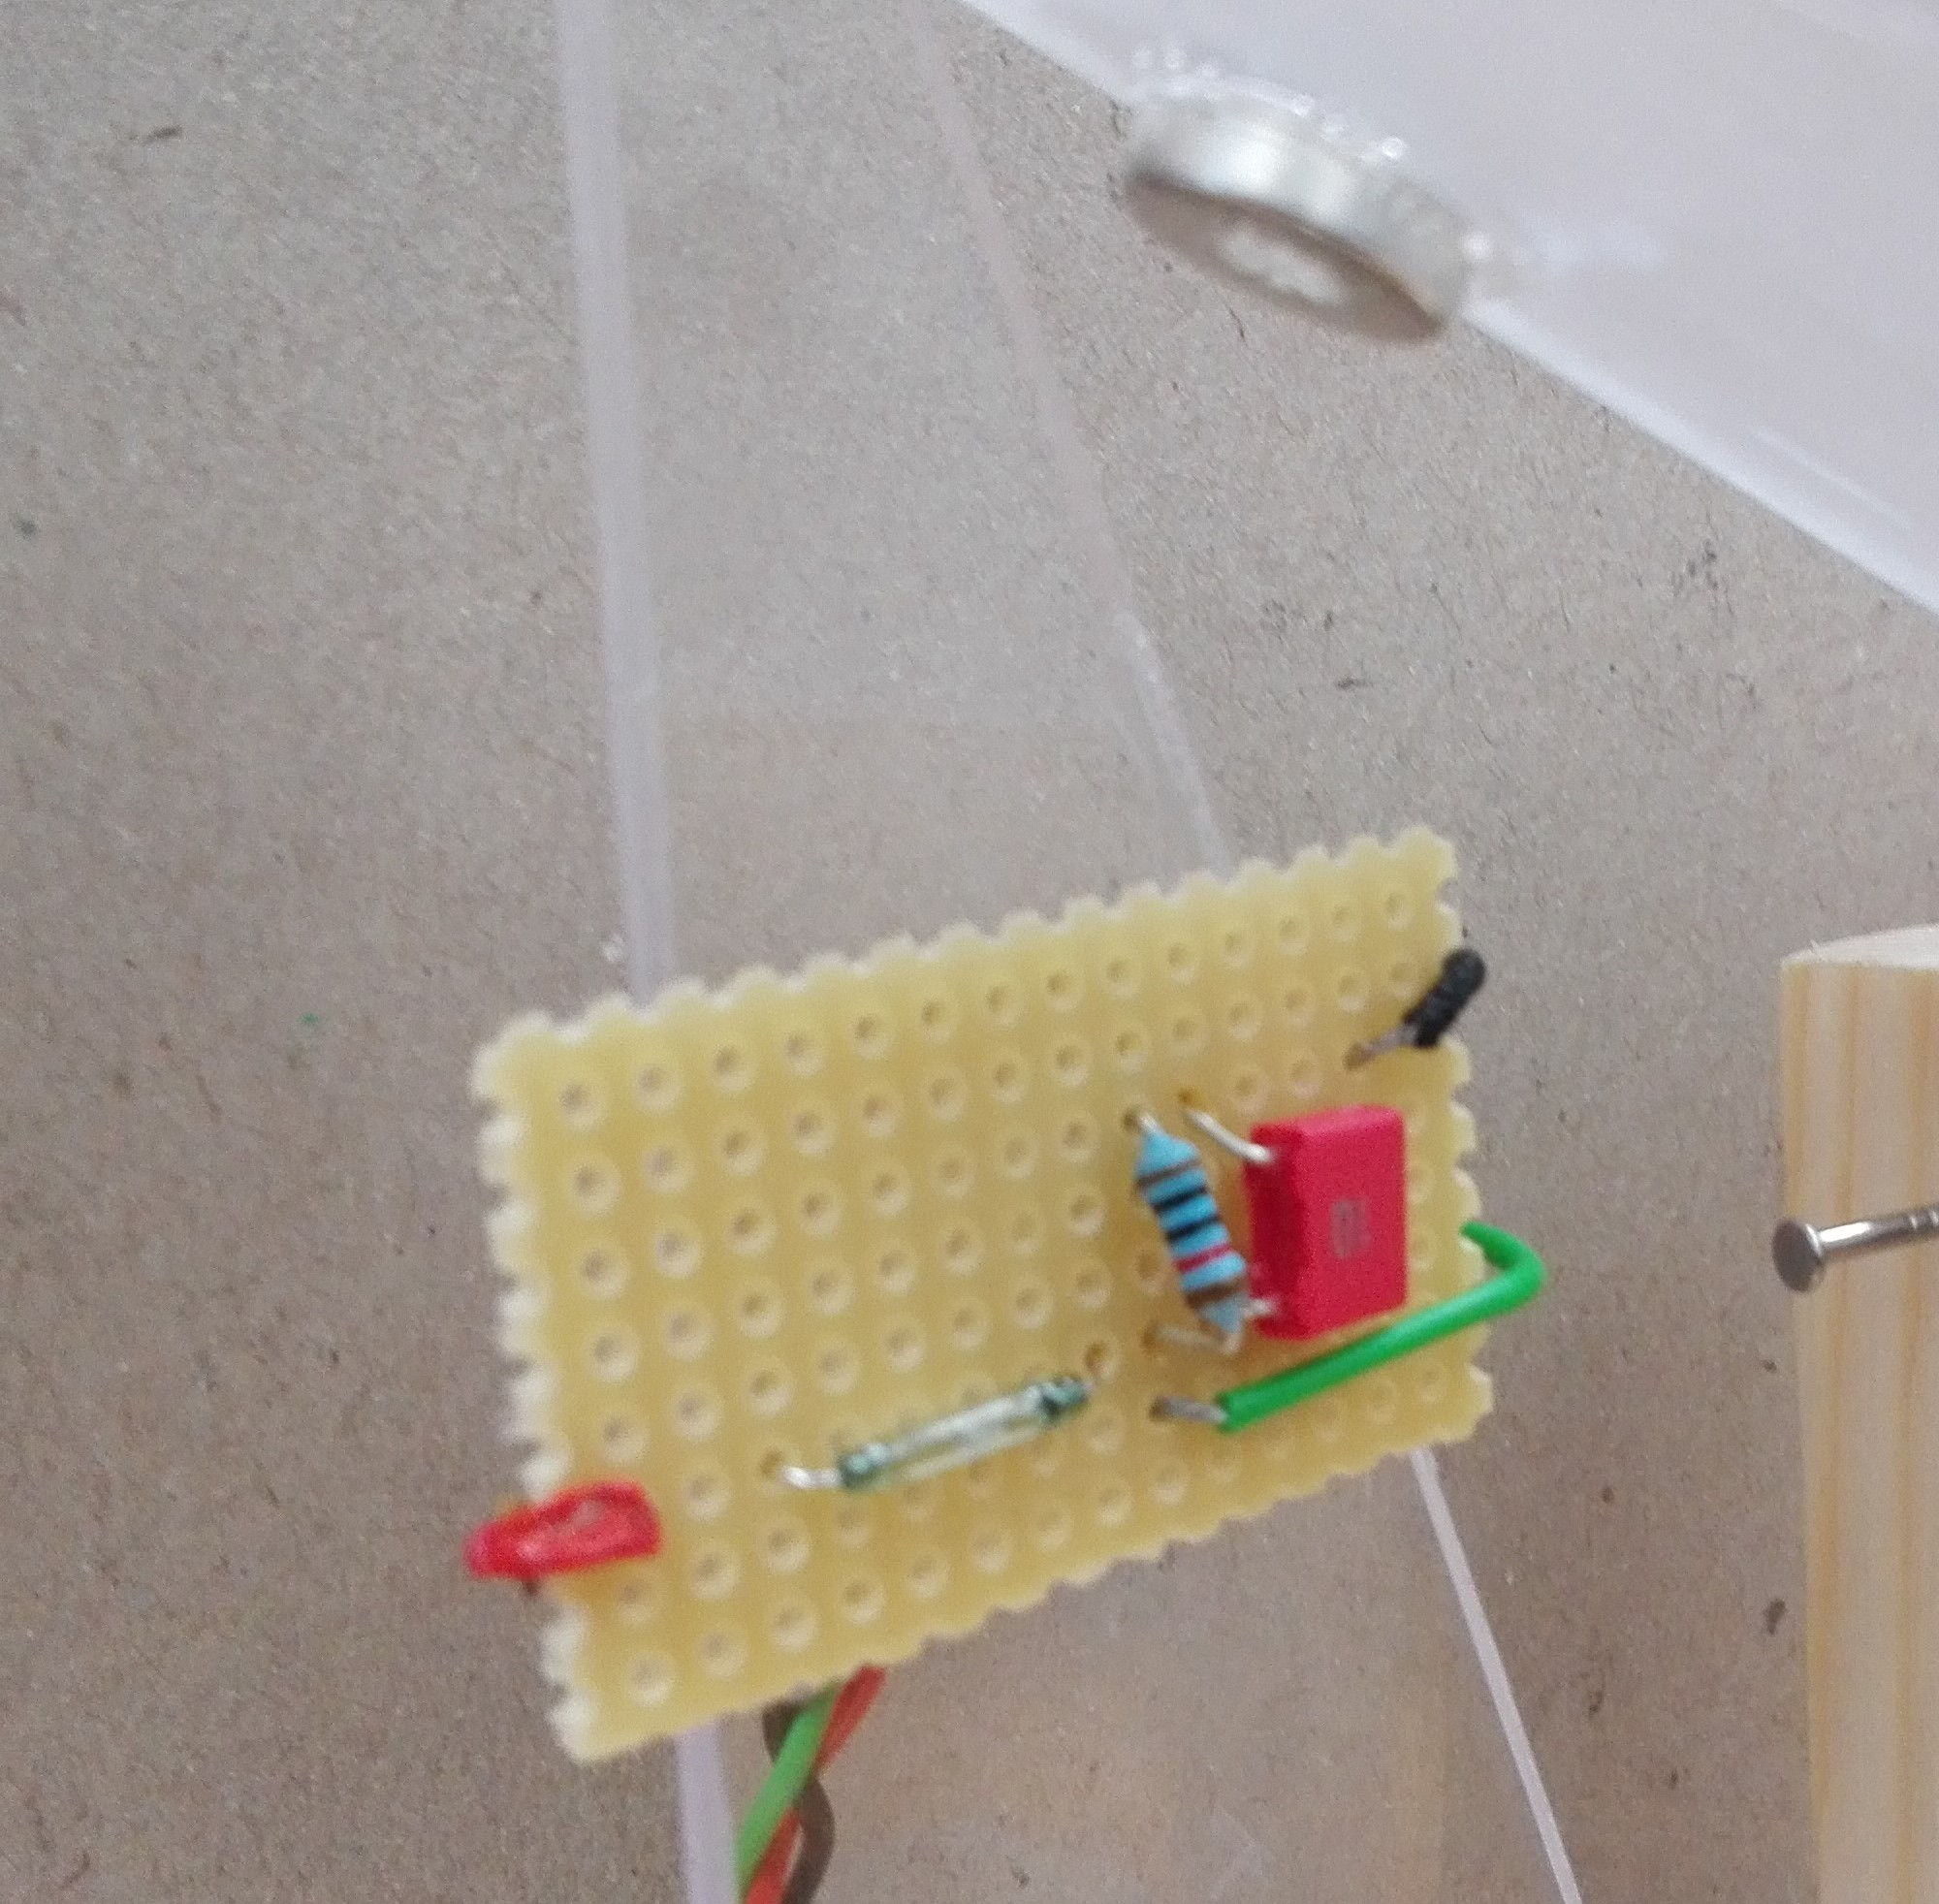
\includegraphics[width=0.35\linewidth]{graphics/KippSchalt.jpg}
\caption{Schaltkreis zur detektion der Kippbewegung.}
\label{fig:KippSchalt}
\end{figure}

Abbildung \ref{fig:KippSchalt} zeigt den Schaltkreis zur detektion der Kippbewegung. Benutzt wurde ein 10k$\Omega$ Widerstand mit einem parallel angeschlossenen 100nF Kondensator. Der Reedkontakt reagiert auf den ebenso sichtbaren Permanentmagneten, welcher an der Unterseite des Kipplöffels befestigt ist.
\newpage
\paragraph{\textbf{Nachteile des Selbstgebauten Niederschlagsmengensensor}}
Der selbstgebaute Niederschlagssensor beweist, dass das Prinzip des Kipplöffels funktioniert. Dennoch weist der Selbstbau Mängel auf. Der verwendete Permanentmagnet muss geklebt werden, weshalb dessen Magnetfeld massiv an stärke verliert und die Schaltung deshalb äusserst nahe angebracht werden muss. Ausserdem kam es, dadurch dass keine Werkstatt zugänglich war, zu Improvisation bei nahezu allen Fertigungsschritten, was zu unkalkulierbaren Abweichungen führt. Als Beispiel sei das Spiel der drehbaren Lagerung des Kipplöffels auf dem Gerüst angeführt, was jegliche Justierungsversuche der Niederschlagsmenge beeinflusst. Aus den genannten Gründen wird vorgefertigter Sensor mit Kipplöffelprinzip verwendet.

\begin{figure}[hbtp]
\centering
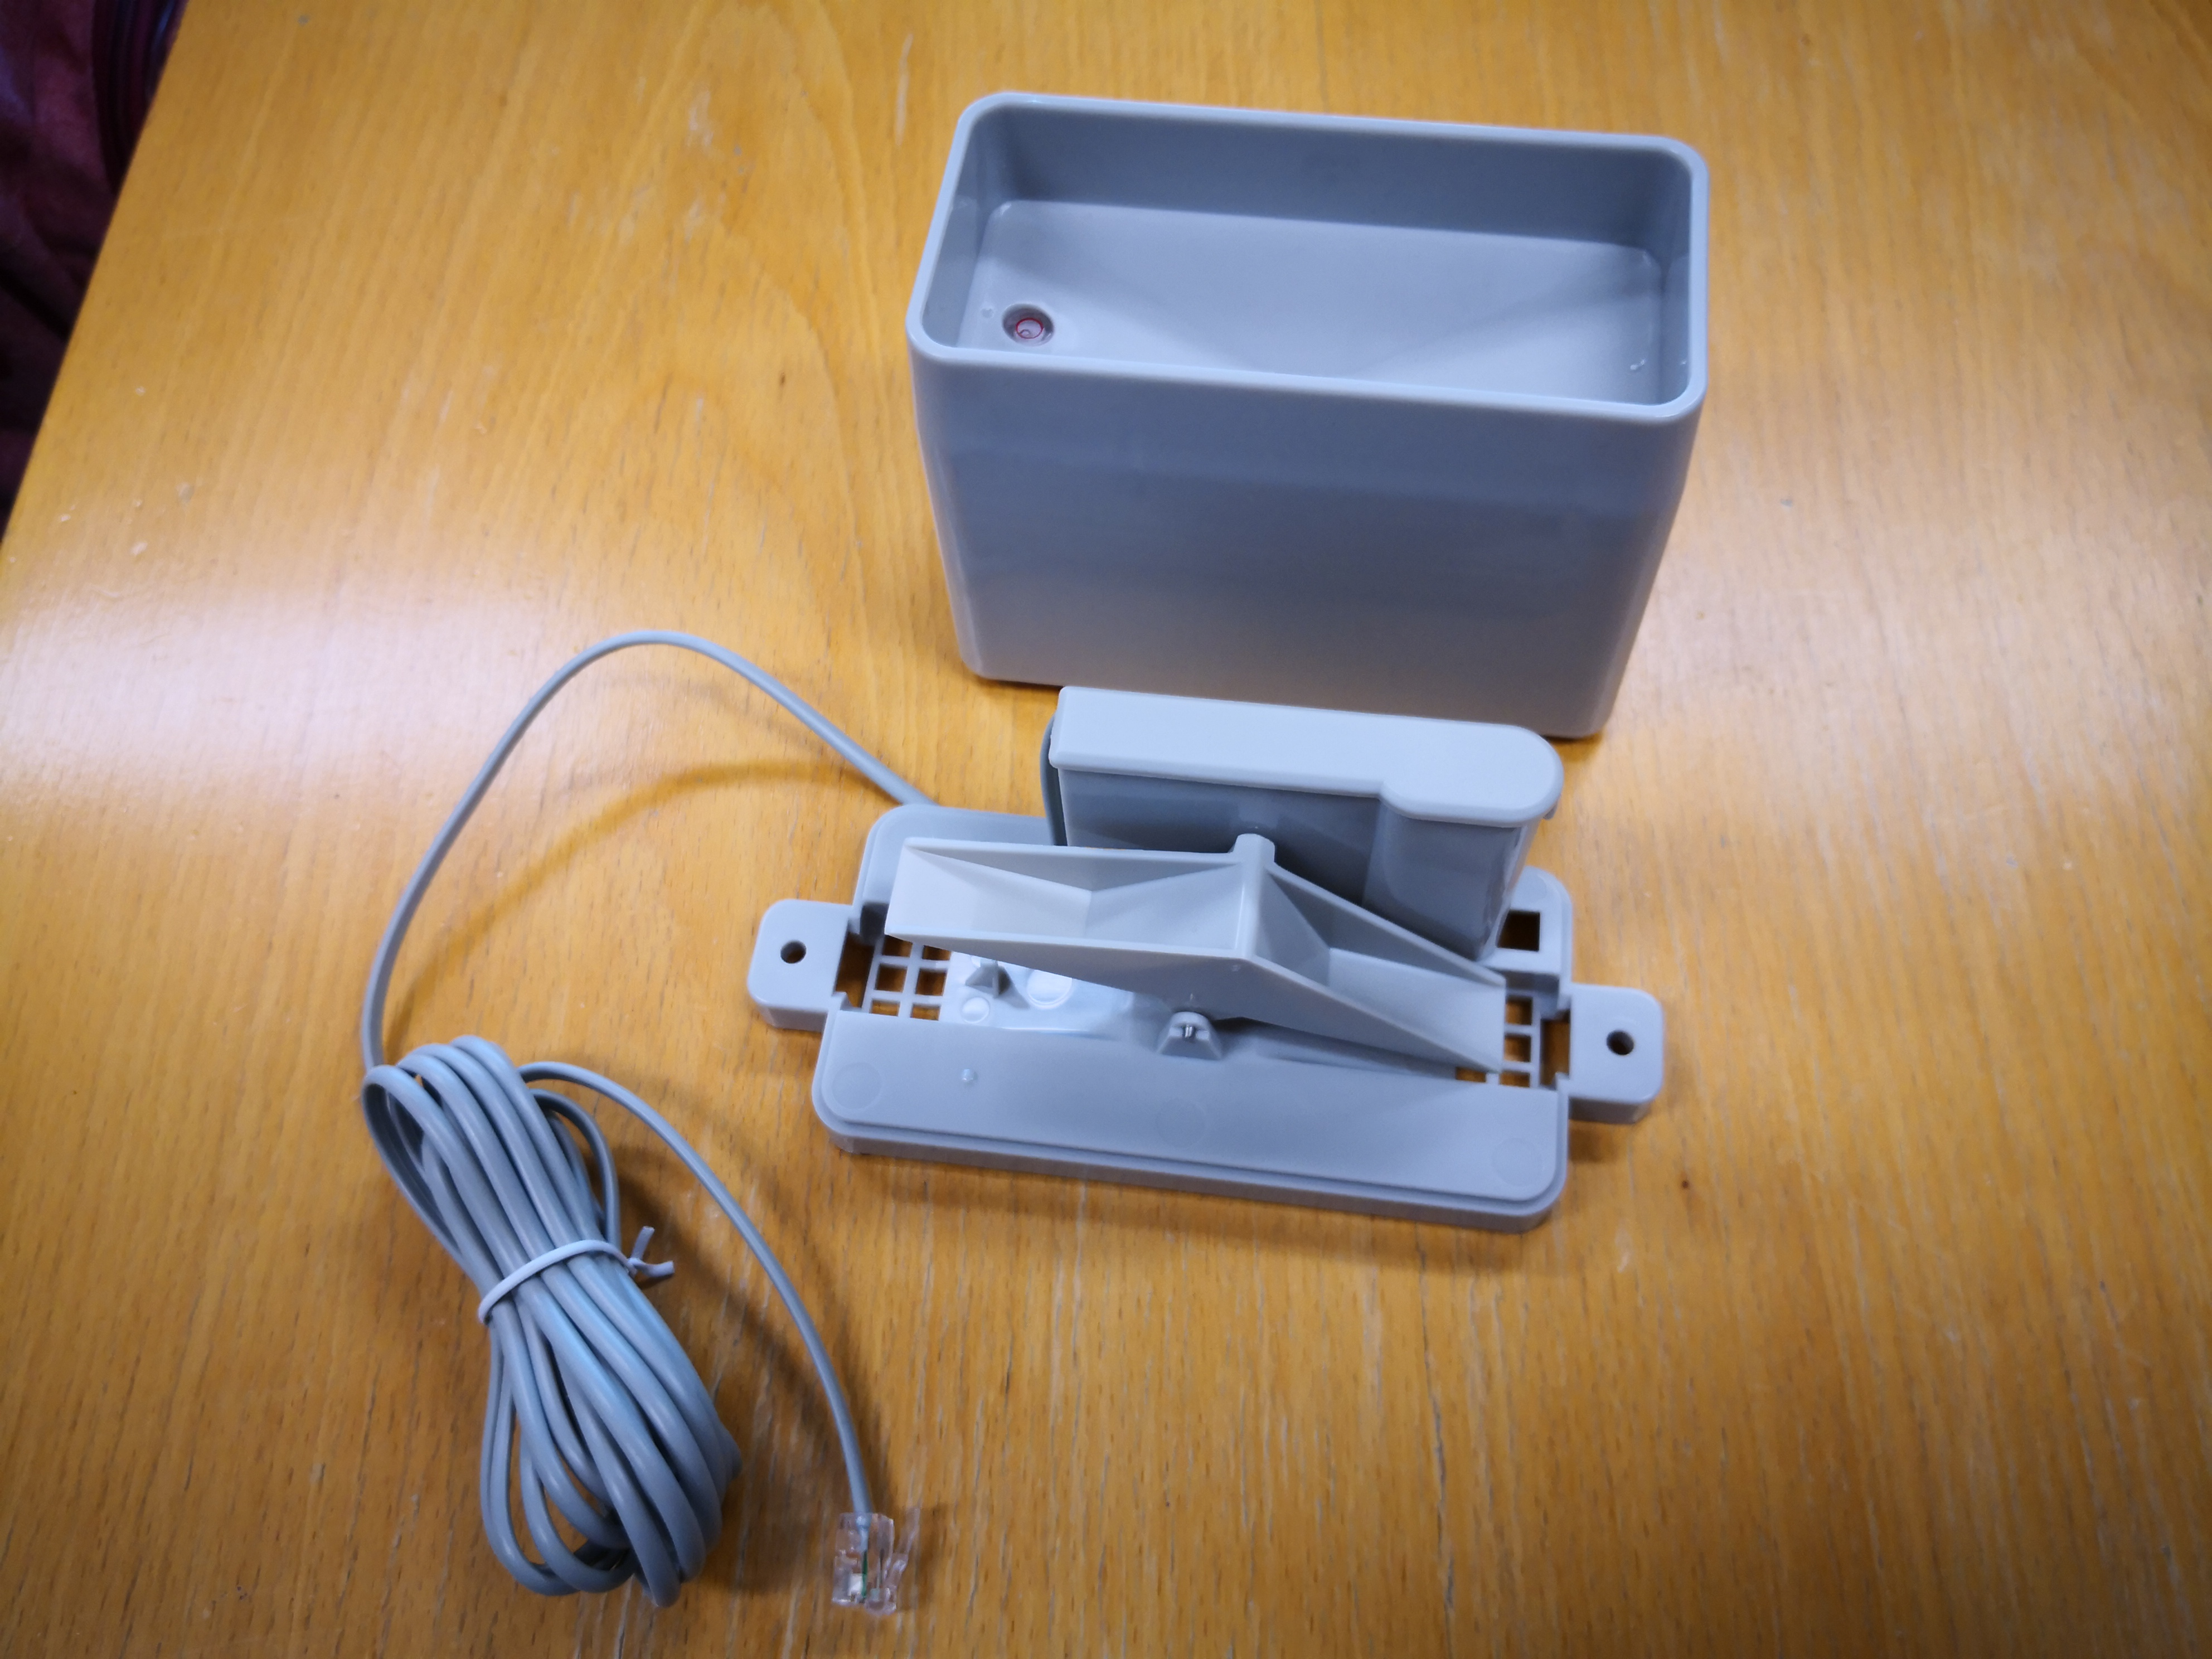
\includegraphics[width=0.7\textwidth]{graphics/ombrometer/IMG_20190118_110027.jpg}
\caption{Das Ombrometer}
\label{fig:verwendetes_ombrometer}
\end{figure}

Das verwendete Ombrometer von MISOL hat eine Auflösung von ca. 2ml pro Kippbewegung auf auf die Dimensionen $5.5E-2m*11.5E-2m$ des Trichters. Zudem enthält der Trichter oben noch eine kleine Wasserwaage, damit das Ombrometer auch gerade steht und die gemessene Regenmenge nicht verfälscht wird.

%\subsubsection*{Implentation in der Firmware}
%Die Implementation wurde über einen Interrupt-Pin des ATMega2560 gemacht. Jedes mal wenn der Kipplöffel des Ombrometers kippt, wird ein Interrupt der auf die steigende Flanke des anliegenden Signals getriggert ist ausgeführt, welcher einen Counter für das Ombrometer inkrementiert. Eine Kippbewegung des Ombrometers umfasst ca. 2ml auf eine Fläche von $5.5E-2m*11.5E-2m=\underline{\underline{6.325E-3m^{2}}}$. Hochgerechnet auf einen Quadratmeter ergibt sich
%\begin{equation}
%2ml*\dfrac{1m^{2}}{6.325E-3m^{2}} = \underline{\underline{316.21ml}}
%\end{equation}
%benötigter Niederschlag für eine Kippbewegung des Ombrometers pro Quadratmeter. Nun kann die Niederschlagmenge in einem bestimmten Zeitraum ausgegeben werden.\\

\subsubsection{Anemometer - Projekt 5}
{\begin{minipage}[b][650pt][t]{0.55\textwidth}
Für die Windgeschwindigkeitsmessung wurde ein Ersatz Anemometer von Froggit genommen (Abb. \ref{fig:anemometer}). Das Anschlusskabel hat einen vier poligen RJ-11 Stecker, dessen Signal über eine Buchse zum MCU geführt wird. Das Anemometer selbst hat allerdings nur zwei Anschlüsse, die Speisung (rot) und das durch einen mit einem Dauermagneten schließbaren Reedkontakt modulierte pulsförmige Ausgangssignal (grün, Abb. \ref{fig:rj11stecker}). In der Abb. \ref{fig:beschaltungAnemometer} ist ersichtlich, dass das Ausgangssignal über R1 abfällt und C1 als Spannungsstabilisierung dient. Das daraus resultierende Signal ist in der Abb. \ref{fig:rechteckpuls_anemometer} aufgezeigt. Die Windgeschwindigkeit ist nun aus der Anzahl Rechteckpulsen direkt interpretierbar:\\

Wenn über einen Zeitraum $T$ die Anzahl Pulse $A$ gemessen werden, dann kann auf die Winkelgeschwindigkeit $\omega$ nach 
\begin{equation}
\centering
\omega=\frac{A}{T}\qquad[s^{-1}]
\end{equation}
geschlossen werden. Da allerdings verschiedene Faktoren wie das Trägheitsmoment des Schalenkreuzes, Reibungsverluste bei der Drehbewegung, Verfälschung bei wechselnder Windrichtung usw. zusätzlich auf das Anemometer wirken, wird es sehr komplex die Windgeschwindigkeit exakt zu berechnen. Deshalb wird nur ein Näherungswert ermittelt und mit einem Skalierungsfaktor $SF$ korrigiert. Somit ergibt sich für die Windgeschwindigkeit $v_{Wind}$ mit Radius $r$ des Schalenkreuzes
\begin{equation}
\centering
v_{Wind} = \frac{A\cdot r\cdot SF}{T}\qquad[m/s].
\label{equ:berechnungWindgeschwindigkeit}
\end{equation}
Der Skalierungsfaktor $SF$ wird mittels Referenzmessungen der Windgeschwindigkeit eines digitalen Anemometers eruiert. \\
\end{minipage}}
{\begin{minipage}[b][650pt][t]{0.44\textwidth}
\centering
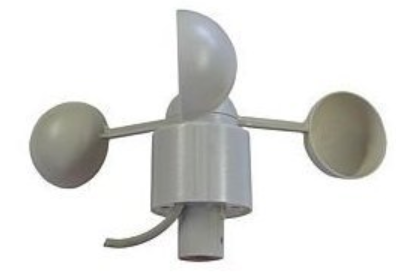
\includegraphics[width=0.9\textwidth]{graphics/Anemometer/anemometer.png}
\captionof{figure}{Anemometer \cite{AmazonAnemometer}}
\label{fig:anemometer}
\vspace{20pt}
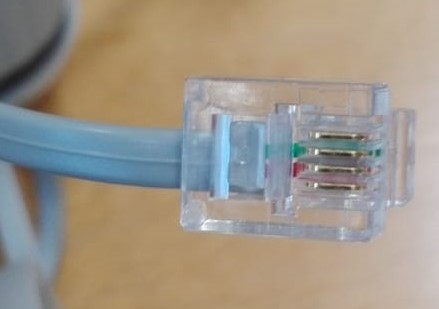
\includegraphics[width=0.9\textwidth]{graphics/Anemometer/rj_11_anschlussstecker.png}
\captionof{figure}{RJ-11 Stecker}
\label{fig:rj11stecker}
\vspace{20pt}
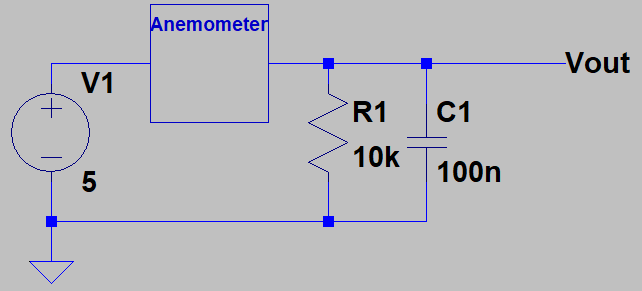
\includegraphics[width=0.9\textwidth]{graphics/Anemometer/schaltung_anemometer.png}
\captionof{figure}{Beschaltung des Ausgangs des Anemometers.}
\label{fig:beschaltungAnemometer}
\vspace{20pt}
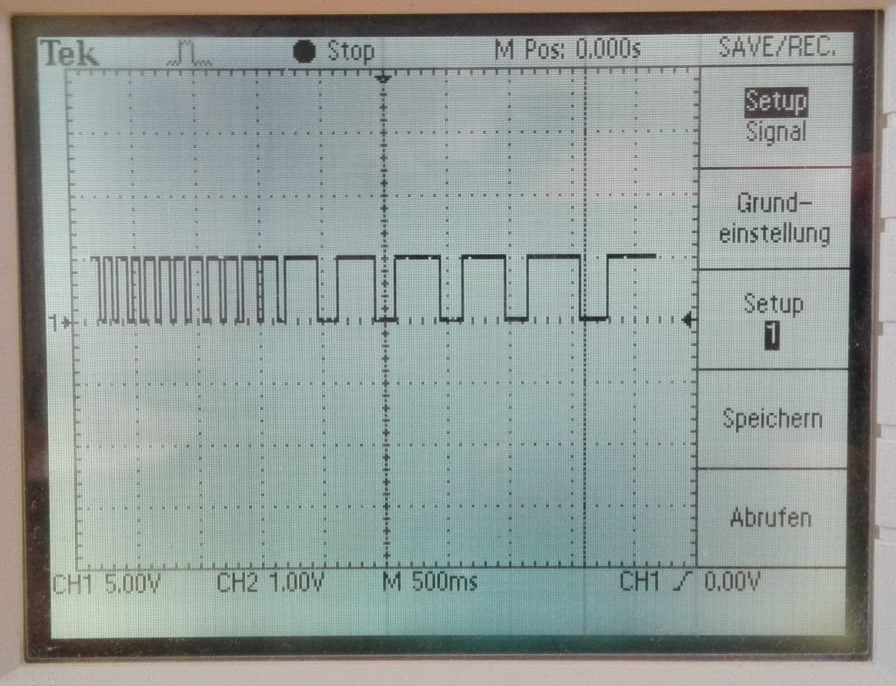
\includegraphics[width = 0.9\textwidth]{graphics/Anemometer/oszilloskop_anenometer_puls.png}
\captionof{figure}{Ausgangssignal $V_{out}$}
\label{fig:rechteckpuls_anemometer}
\end{minipage}}
\newpage

%\subsubsection*{Implementation in die Firmware}
%Die Implementation wurde recht simpel gehalten. Der gesamte implementierte Code für das Anemometer ist im Headerfile ''Anemometer.h'' extern deklariert und im File Anemometer.cpp initialisiert. Das Signal $V_{out}$ ist mit einen digital Pin des Atmega 2560 (Pinnummer 2 des Arduino Mega Boards) verbunden. Über einen Zeitraum von $5000ms$, auf die steigende Flanke getriggert, wird die Anzahl von Pulsen mittels Interrupt\footnote{es handelt sich hierbei um \textit{external Interrupts}.} gezählt. Dabei wird zuerst der Interrupt auf der Pinnummer 2 aktiviert, mit einem Delay von $5000ms$ gewartet, wobei bei jedem ausgelösten Interrupt die Funktion \textcolor{orange}{countWind}() ausgeführt und somit bei jeder steigenden Flanke um eins inkrementiert wird. Zum Schluss folgt die Deaktivierung des Interrupts und die Berechnung der Windgeschwindigkeit nach der Gleichung \ref{equ:berechnungWindgeschwindigkeit}.\\

\subsubsection{Windrichtungsgeber - Projekt 5}
{\begin{minipage}[b][10cm][t]{0.55\textwidth}
Um die Windrichtung angeben zu können, wurde ein Windrichtungsgeber, wie in Abb. \ref{fig:windrichtungsgeber} gezeigt von MISOL verwendet. Er ist genau wie das Ombrometer und das Anemometer mit Reedkontakten realisiert worden (siehe Abb. \ref{fig:interne_schaltung}). Dafür sind acht Reedkontakte im Kreis angeordnet und jeder hat einen in Serie geschalteten Widerstand von unterschiedlichen Dimensionen. Der Dauermagnet kann, je nach Drehwinkel bis zu zwei Reedkontakte gleichzeitig schließen. Dies erlaubt sechzehn verschiedene Winkelpositionen und somit eine Auflösung von 22.5$^{o}$. Mit einem externen Widerstand $R=10k\Omega$ (siehe Abb. \ref{fig:aussere_beschaltung}) wird eine Spannung generiert, welche dann mit dem ADC des Microcontrollers gelesen werden kann. Der Windrichtungsgeber wird mit einer Speisespannung von $V_{+}=5V$ betrieben. Der Windrichtungsgeber hat einen vierpoligen RJ-11 Anschluss. Zudem hat er auf der unteren Seite noch eine RJ-11 Buchse, bei der das Anemometer direkt angeschlossen werden kann. Wie diese Anschlüsse gemapped sind, wird in der Abb. \ref{fig:interne_schaltung} gezeigt. \\
\end{minipage}}
{\begin{minipage}[b][10cm][t]{0.44\textwidth}
\centering
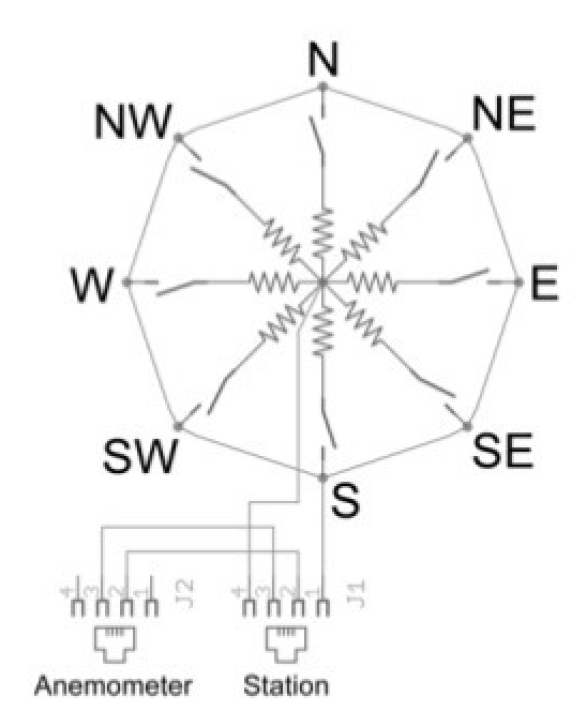
\includegraphics[width=0.9\textwidth]{graphics/windrichtungsgeber/interne_schaltung.PNG}
\captionof{figure}{Interne Schaltung \cite{ADSkeineAngabe}}
\label{fig:interne_schaltung}
\end{minipage}}

\begin{table}[h]
\centering
\caption{Technische Werte \cite{ADSkeineAngabe}}
\begin{tabular}{|c|c|c|c|}
\hline 
Richtung [$^{o}$] & Himmelsrichtung & Widerstand [$\Omega$] & Ausgangsspannung [V] \\ 
\hline 
0 & N & 33k & 3.84 \\ 
\hline 
22.5 &  & 6.57k & 1.98 \\ 
\hline 
45 & NE & 8.2k & 2.25 \\ 
\hline 
67.5 &  & 891 & 0.41 \\ 
\hline 
90 & E & 1k & 0.45 \\ 
\hline 
112.5 &  & 688 & 0.32 \\ 
\hline 
135 & SE & 2.2k & 0.90 \\ 
\hline 
157.5 &  & 1.41k & 0.62 \\ 
\hline 
180 & S & 3.9k & 1.40 \\ 
\hline 
202.5 &  & 3.14k & 1.19 \\ 
\hline 
225 & SW & 16k & 3.08 \\ 
\hline 
247.5 &  & 14.12k & 2.93 \\ 
\hline 
270 & W & 120k & 4.62 \\ 
\hline 
292.5 &  & 42.12k & 4.04 \\ 
\hline 
315 & NW & 64.9k & 4.33 \\ 
\hline 
337.5 &  & 21.88k & 3.43 \\ 
\hline 
\end{tabular} 
\label{tab:technische_werte}
\end{table}

In der Tabelle \ref{tab:technische_werte} sind die Widerstandswerte der in Abb. \ref{fig:interne_schaltung} gezeigten Widerständen und die Werte der Ausgangsspannung bei variabler Winkelposition aufgelistet. Da nun abhängig von der Winkelposition unterschiedliche Widerstände parallel geschalten werden, resultiert am Ausgang eine vom Winkel abhängige Ausgangsspannung.\\

\newpage


{\begin{minipage}[b][6cm][t]{0.49\textwidth}
\centering
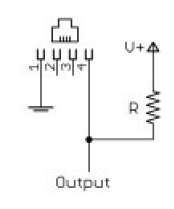
\includegraphics[width=0.5\textwidth]{graphics/windrichtungsgeber/aeussere_beschaltung.PNG} 
\captionof{figure}{Spannungsteiler mit $R=10k\Omega$ \cite{ADSkeineAngabe}}
\label{fig:aussere_beschaltung}
\end{minipage}}
{\begin{minipage}[b][6cm][t]{0.49\textwidth}
\centering
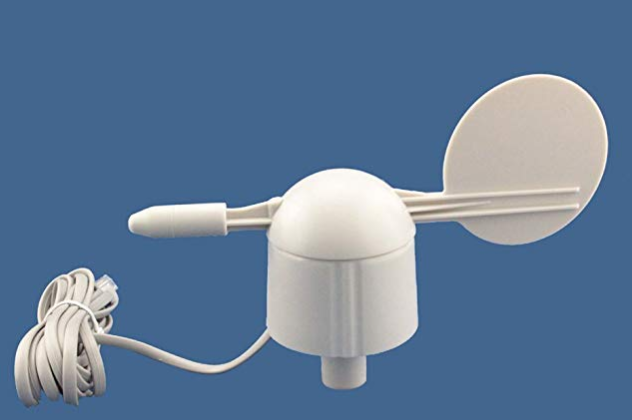
\includegraphics[width=0.9\textwidth]{graphics/windrichtungsgeber/windrichtungsgeber.PNG}
\captionof{figure}{Windrichtungsgeber von MISOL \cite{windrichtungsgeber}}
\label{fig:windrichtungsgeber}
\end{minipage}}

%\subsubsection*{Implementation in die Firmware}
%Der ADC hat des ATMega2560 hat eine 10 Bit Auflösung und wird mit 5 Volt betrieben. Um das Signal am ADC lesen zu können, wird die Funktion \textit{analogRead()} aufgerufen. Als Rückgabewert wird ein binärer Wert als Dezimalzahl vom Datentyp \textit{float} erhalten. Um diesen Wert in die eigentlich am ADC anliegende Spannung umzurechnen wird die Gleichung \ref{equ:ADC1} umgeformt.
%\begin{equation}
%\centering
%\dfrac{Auflösung ADC}{Betriebsspannung} = \dfrac{analogRead()}{Ausgangsspannung}
%\label{equ:ADC1}
%\end{equation}
%Daraus resultiert:
%\begin{equation}
%\centering
%Ausgangsspannung = \dfrac{analogRead()*Betriebsspannung}{Auflösung ADC}
%\label{equ:ADC2}
%\end{equation}
%Werden nun die Werte in die Gleichung \ref{equ:ADC2} eingefügt, ergibt sich für die Ausgangsspannung $V_{out}$:
%\begin{equation}
%\centering
%V_{out}(analogRead()) = \dfrac{analogRead()*5V}{10}
%\label{equ:adc_vout}
%\end{equation}
%Diese von \textit{analogRead()} abhängige Ausgangsspannung $V_{out}$ wird dann in \textit{if else} Anweisungen zu der Himmelsrichtung zugewiesen und als String abgespeichert.

\subsubsection{BME280 - Projekt 5}
\label{BME280}
{\begin{minipage}[b][6cm][t]{0.55\textwidth}
Der \textit{BME280} ist ein low powered digitaler Feuchtigkeits-, Luftdruck- und Temperatursensor von Bosch. Er ist in einem 2.5mm x 2.5mm x 0.93mm metal lid LGA Gehäuse verpackt und kann über die Interfaces I$^{2}$C und SPI kommunizieren. Durch seinen niedrigen Stromverbrauch, große operating range der drei Messgrößen und schnellen Ansprechzeit von etwa 1s eignet er sich für die solarbetriebene mobile Wetterstation besonders. \cite{Bosch2019}\\
\end{minipage}}
{\begin{minipage}[b][6cm][t]{0.44\textwidth}
\centering
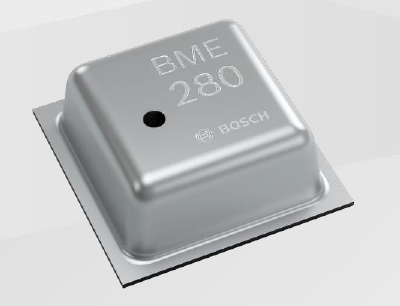
\includegraphics[width=0.9\textwidth]{graphics/bme280/bme280.PNG}
\captionof{figure}{BME280 \cite{Bosch2019}}
\label{fig:bme280}
%\vspace*{0.5cm}
%\centering
%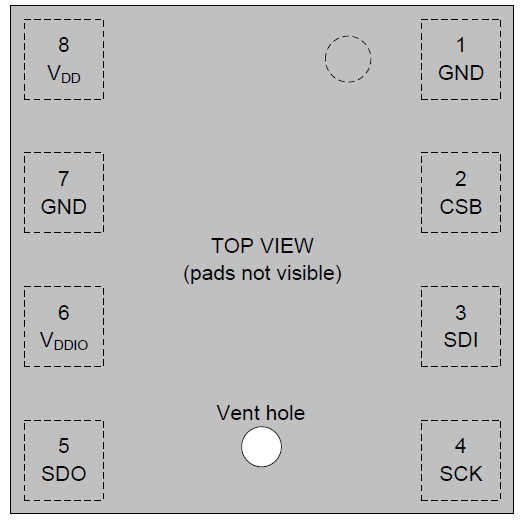
\includegraphics[width=0.9\textwidth]{graphics/bme280/bme280_pinout.PNG}
%\captionof{figure}{Pinout \cite{Bosch2019}}
%\label{fig:bme280_pinout}
\end{minipage}}

\begin{table}[h]
  \centering
  \caption{Elektrische Spezifikationen \cite{Bosch2019}}
    \begin{tabular}{lllll}
    \toprule
    \textbf{Parameter} & \textbf{Min.} & \textbf{Typ.} & \textbf{Max.} & \textbf{Einheit} \\
    \midrule
    Versorgungsspannung & 1.71  & 1.8   & 3.6   & V \\
    Stromverbrauch (sleep mode) &       & 0.1   & 0.3   & $\mu$A \\
    Stromverbrauch inaktiv (normal mode) &       & 0.2   & 0.5   & $\mu$A \\
    Stromverbrauch Feuchtigkeitsmessung &       & 340   &       & $\mu$A \\
    Stromverbrauch Luftdruckmessung &       & 714   &       & $\mu$A \\
    Stromverbrauch Temperaturmessung &       & 350   &       & $\mu$A \\
    \bottomrule
    \end{tabular}%
  \label{tab:elektrische_Spezifikationen}%
\end{table}%

Bei einer Messfrequenz von 1Hz für die drei Messgrößen verbraucht der BME280 somit laut Datenblatt nur \textbf{3.6$\mu$A}. \cite[S. 2]{Bosch2019}

\subsubsection*{\textbf{Feuchtigkeitsmessung}}
In der Tabelle \ref{tab:spez_feuchtigkeit} sind die wichtigsten Parameter zur Feuchtigkeitsmessung aufgelistet. Zu vermerken ist, dass die digitalen Werte des BME280 zur Feuchtigkeitsmessung relativ sind und deshalb prozentual angegeben werden. \\
\begin{table}[htbp]
  \centering
  \caption{Sezifikationen der Feuchtigkeitsmessung \cite{Bosch2019}}
    \begin{tabular}{lllll}
    \toprule
     \textbf{Parameter} & \textbf{Min.} & \textbf{Typ.} & \textbf{Max.} & \textbf{Einheit} \\
    \midrule
    Operating range & -40   & 25    & 85    & $^{o}$C \\
          & 0     &       & 100   & \% \\
    Absolute Genauigkeitstoleranz &       & $\pm$3 &       & \% \\
    Hysterese &       & $\pm$1 &       & \% \\
    Auflösung &       & 0.008 &       & \% \\
    Langzeitstabilität &       & 0.5   &       & \% pro Jahr \\
    \bottomrule
    \end{tabular}%
  \label{tab:spez_feuchtigkeit}%
\end{table}%

\newpage

\subsubsection*{\textbf{Luftdruckmessung}}
Die Genauigkeit der Luftdruckmessung ist an einen Temperaturbereich gebunden. Bei niedrigeren Temperaturen (<0$^{o}$C) weist der Sensor eine höhere Unsicherheit auf als bei Temperaturen von 0 bis 65 $^{o}$C (siehe Tabelle \ref{tab:spez_druck}). \\
\begin{table}[htbp]
  \centering
  \caption{Sezifikationen der Luftdruckmessung \cite{Bosch2019}}
    \begin{tabular}{llllll}
    \toprule
    \textbf{Parameter} & \multicolumn{1}{l}{\textbf{Temperaturbereich}} & \multicolumn{1}{l}{\textbf{Min.}} & \textbf{Typ. } & \multicolumn{1}{l}{\textbf{Max.}} & \textbf{Einheit} \\
    \midrule
    Operating range &       & \multicolumn{1}{l}{-40} & 25    & \multicolumn{1}{l}{85} & $^{o}$C \\
          &       & 300   &       & 1100  & hPa \\
    Absolute Genauigkeit & \multicolumn{1}{c}{-20 bis 0 $^{o}$C} &       & $\pm$1.7 &       & hPa \\
          & \multicolumn{1}{c}{0 bis 65 $^{o}$C} &       & $\pm$1  &       & hPa \\
    Auflösung &       &       & \multicolumn{1}{r}{0.18} &       & hPa \\
    Langzeitstabilität &       &       & $\pm$1  &       & hPa pro Jahr \\
    \bottomrule
    \end{tabular}%
  \label{tab:spez_druck}%
\end{table}%

\subsubsection*{\textbf{Temperaturmessung}}
Die Wetterstation wird hauptsächlich in einem Temperaturbereich von 0 bis 65 $^{o}$C betrieben, wodurch vom Sensor eine Unsicherheit von max. $\pm$1 $^{o}$C erreicht werden kann. \\
\begin{table}[htbp]
  \centering
  \caption{Sezifikationen der Temperaturmessung \cite{Bosch2019}}
    \begin{tabular}{llllll}
    \toprule
    \textbf{Parameter} & \multicolumn{1}{l}{\textbf{Temperaturbereich}} & \multicolumn{1}{l}{\textbf{Min.}} & \textbf{Typ. } & \multicolumn{1}{l}{\textbf{Max.}} & \textbf{Einheit} \\
    \midrule
    Operating range &       & \multicolumn{1}{l}{-40} & 25    & \multicolumn{1}{l}{85} & $^{o}$C \\
    Absolute Genauigkeit & \multicolumn{1}{c}{25 C} &       & $\pm$0.5 &       & $^{o}$C \\
          & \multicolumn{1}{c}{0 bis 65 C} &       & $\pm$1  &       & $^{o}$C \\
          & \multicolumn{1}{c}{-20 bis 0 C} &       & $\pm$1.25 &       & $^{o}$C \\
          & \multicolumn{1}{c}{-40 bis -20 C} &       & $\pm$1.5 &       & $^{o}$C \\
    Auflösung  &       &       & 0.01  &       & $^{o}$C \\
    \bottomrule
    \end{tabular}%
  \label{tab:spez_temp}%
\end{table}%

%\subsubsection*{Implementation in die Firmware}
%Um den BME280 vom Microcontroller aus ansteuern zu können, wurden zwei bereits existierende Librarys von Adafruit verwendet:
%\begin{itemize}
%\item Adafruit BME280 Library
%\item Adafruit Unified Sensors
%\end{itemize}
%Anschließend konnten die Headerfiles <Adafruit\_Sensor.h> und <Adafruit\_BME280.h> inkludiert werden und der Sensor über das I$^{2}$C Interface mit den folgenden Funktionen abgefragt werden:\\
%\begin{itemize}
%\item \textcolor{blue}{float} \textcolor{orange}{readTemperature}()
%\item \textcolor{blue}{float} \textcolor{orange}{readHumidity}()
%\item \textcolor{blue}{float} \textcolor{orange}{readPressure}()
%\end{itemize}

\subsection{Ergänzungen aus der Bachelor-Thesis}
Während der Bachelor-Thesis soll ein Sensor zur Ermittlung der Sonnenstunden implementiert werden. Um dies zu erreichen wurde die Idee, die Sonnenstunden direkt über den Ladestrom der Photovoltaikanlage zu eruieren, verworfen, da auf diese Weise mit höheren Energieverlusten zu rechnen wäre durch das Abzweigen des Ladestroms und die damit verbundene zusätzliche Speisung der zusätzlichen Schaltung. Stattdessen wird über ein Lichtintensitätssensor die Bestrahlungsstärke gemessen, womit die Sonnenstunden über einen Schwellwert berechnet werden können. Im folgenden Abschnitt wird der verwendete Lichtintensitätssensor näher erläutert.

\subsubsection{Lichtintensitätssensor}
Die Lichtintensität wird über den TSL2561, ein digitaler low power Sensor, eruiert. Dieser misst über eine Kombination aus einer Breitband-Photodiode und einer Infrarot-Photodiode die Lichtstärke mit einer 16-Bit Auflösung. Über zwei integrierte AD-Wandler wird der Photodiodenstrom gewandelt und auf einen digitalen Ausgang gegeben. Über eine I$^{2}$C Schnittstelle kann dieser Ausgang auf die MCU gegeben und so ausgewertet werden. Ab einem bestimmten Schwellenwert kann die Einstrahlung als direkte Sonnenstrahlung definiert, und so auch gezählt werden. Der erwähnte Schwellwert ist vom Ort abhängig an dem die Wetterstation sich befindet und muss eruiert und in der Firmware eingestellt werden, was im entsprechenden Teil (\refname{part:Firmware} \ref{part:Firmware})) erläutert wird. Da dieser Sensor nicht direkt auf der Platine sondern am oberen Teil des Gehäuses montiert werden muss, wird der TSL2561 als Breakout Board (Abbildung \ref{fig:TSL}) verwendet und über Pinheader mit dem PCB verbunden. Die wichtigsten elektrischen Spezifikationen sind in der Tabelle \ref{tab:TSL2561} zusammengefasst. \cite{TSL2561}\\

\begin{figure}[hbtp]
\centering
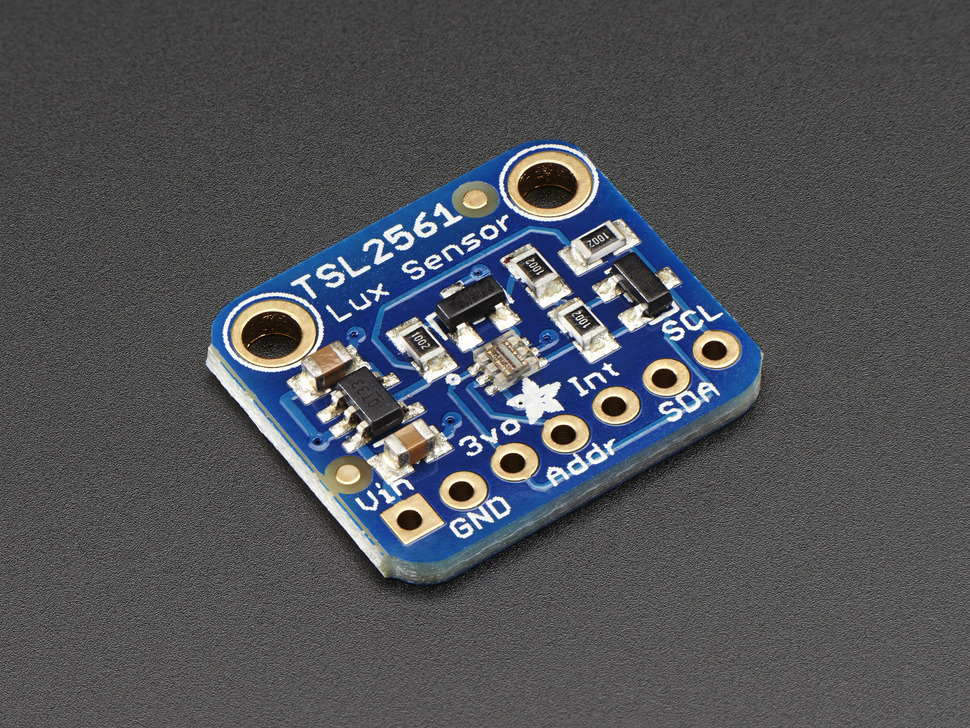
\includegraphics[width=0.5\textwidth]{graphics/TSL2561/TSL2561_Breakout.JPG}
\captionof{figure}{TSL2561 Breakout Board von Adafruit \cite{TSL2561Adafruit}}
\label{fig:TSL}
\end{figure}

\begin{table}[h]
  \centering
  \caption{Elektrische Spezifikationen des TSL2561 \cite{TSL2561}}
    \begin{tabular}{lllll}
    \toprule
    \textbf{Parameter} & \textbf{Min.} & \textbf{Typ.} & \textbf{Max.} & \textbf{Einheit} \\
    \midrule
    Versorgungsspannung & 2.7  & 3   & 3.6   & V \\
    Stromverbrauch (Aktiv) &       & 0.24   & 0.6   & mA \\
    Stromverbrauch inaktiv (Power down) &       & 3.2   & 15 & $\mu$A \\
    \bottomrule
    \end{tabular}%
  \label{tab:TSL2561}%
\end{table}%
\newpage
\subsubsection{BME280}
Im Verlauf der Bachelor-Thesis wurde über das Design des Gehäuses der Wetterstation diskutiert, dabei wurde ebenfalls die Notwendigkeit eines Zugangs zu frischer Umgebungsluft für den BME280 erwähnt. Würde der BME280 auf dem PCB angebracht werden, so würde dieser durch die Abwärme der Elektronik stärker beeinflusst und Fehlmessungen generieren. Aus diesem Grund soll der BME280 an der unteren Seite des Gehäuses, zugänglich zu frischer Aussenluft, montiert werden. Damit Fehlmessungen möglichst vermieden werden können, wird wie beim TSL2561 für den BME280 ein Breakout Board verwendet (Abbildung \ref{fig:BME_Breakout}) und über Pinheader mit dem PCB verbunden.\\

\begin{figure}[hbtp]
\centering
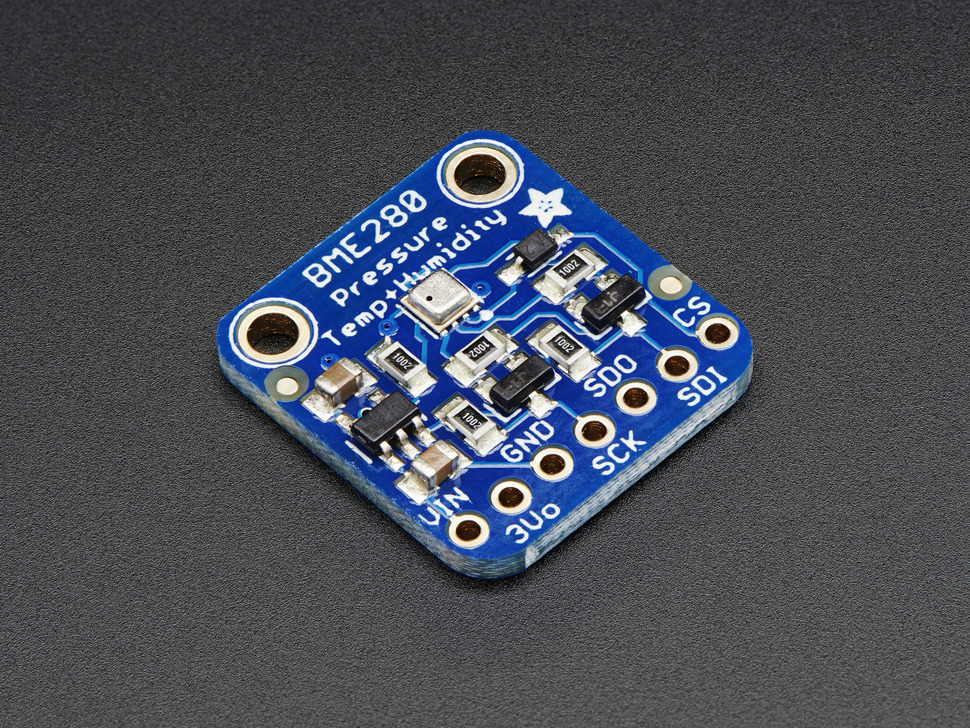
\includegraphics[width=0.5\textwidth]{graphics/BME280/BME280_Breakout.JPG}
\captionof{figure}{BME280 Breakout Board von Adafruit \cite{BME_Breakout}}
\label{fig:BME_Breakout}
\end{figure}

Die gesammelten Daten der Sensorik werden an die MCU geliefert. Die MCU kann jedoch nicht alle Daten speichern, weshalb ein grösserer, externer Speicher notwendig ist. Aus diesem Grund wird im nächsten Kapitel auf die Datenspeicherung eingegangen.